% Options for packages loaded elsewhere
\PassOptionsToPackage{unicode}{hyperref}
\PassOptionsToPackage{hyphens}{url}
\PassOptionsToPackage{dvipsnames,svgnames,x11names}{xcolor}
%
\documentclass[
  a4paper,
  DIV=11,
  numbers=noendperiod]{scrartcl}

\usepackage{amsmath,amssymb}
\usepackage{iftex}
\ifPDFTeX
  \usepackage[T1]{fontenc}
  \usepackage[utf8]{inputenc}
  \usepackage{textcomp} % provide euro and other symbols
\else % if luatex or xetex
  \usepackage{unicode-math}
  \defaultfontfeatures{Scale=MatchLowercase}
  \defaultfontfeatures[\rmfamily]{Ligatures=TeX,Scale=1}
\fi
\usepackage{lmodern}
\ifPDFTeX\else  
    % xetex/luatex font selection
\fi
% Use upquote if available, for straight quotes in verbatim environments
\IfFileExists{upquote.sty}{\usepackage{upquote}}{}
\IfFileExists{microtype.sty}{% use microtype if available
  \usepackage[]{microtype}
  \UseMicrotypeSet[protrusion]{basicmath} % disable protrusion for tt fonts
}{}
\makeatletter
\@ifundefined{KOMAClassName}{% if non-KOMA class
  \IfFileExists{parskip.sty}{%
    \usepackage{parskip}
  }{% else
    \setlength{\parindent}{0pt}
    \setlength{\parskip}{6pt plus 2pt minus 1pt}}
}{% if KOMA class
  \KOMAoptions{parskip=half}}
\makeatother
\usepackage{xcolor}
\usepackage[top=20mm,bottom=20mm,left=20mm,right=20mm,heightrounded]{geometry}
\setlength{\emergencystretch}{3em} % prevent overfull lines
\setcounter{secnumdepth}{-\maxdimen} % remove section numbering
% Make \paragraph and \subparagraph free-standing
\ifx\paragraph\undefined\else
  \let\oldparagraph\paragraph
  \renewcommand{\paragraph}[1]{\oldparagraph{#1}\mbox{}}
\fi
\ifx\subparagraph\undefined\else
  \let\oldsubparagraph\subparagraph
  \renewcommand{\subparagraph}[1]{\oldsubparagraph{#1}\mbox{}}
\fi

\usepackage{color}
\usepackage{fancyvrb}
\newcommand{\VerbBar}{|}
\newcommand{\VERB}{\Verb[commandchars=\\\{\}]}
\DefineVerbatimEnvironment{Highlighting}{Verbatim}{commandchars=\\\{\}}
% Add ',fontsize=\small' for more characters per line
\usepackage{framed}
\definecolor{shadecolor}{RGB}{241,243,245}
\newenvironment{Shaded}{\begin{snugshade}}{\end{snugshade}}
\newcommand{\AlertTok}[1]{\textcolor[rgb]{0.68,0.00,0.00}{#1}}
\newcommand{\AnnotationTok}[1]{\textcolor[rgb]{0.37,0.37,0.37}{#1}}
\newcommand{\AttributeTok}[1]{\textcolor[rgb]{0.40,0.45,0.13}{#1}}
\newcommand{\BaseNTok}[1]{\textcolor[rgb]{0.68,0.00,0.00}{#1}}
\newcommand{\BuiltInTok}[1]{\textcolor[rgb]{0.00,0.23,0.31}{#1}}
\newcommand{\CharTok}[1]{\textcolor[rgb]{0.13,0.47,0.30}{#1}}
\newcommand{\CommentTok}[1]{\textcolor[rgb]{0.37,0.37,0.37}{#1}}
\newcommand{\CommentVarTok}[1]{\textcolor[rgb]{0.37,0.37,0.37}{\textit{#1}}}
\newcommand{\ConstantTok}[1]{\textcolor[rgb]{0.56,0.35,0.01}{#1}}
\newcommand{\ControlFlowTok}[1]{\textcolor[rgb]{0.00,0.23,0.31}{#1}}
\newcommand{\DataTypeTok}[1]{\textcolor[rgb]{0.68,0.00,0.00}{#1}}
\newcommand{\DecValTok}[1]{\textcolor[rgb]{0.68,0.00,0.00}{#1}}
\newcommand{\DocumentationTok}[1]{\textcolor[rgb]{0.37,0.37,0.37}{\textit{#1}}}
\newcommand{\ErrorTok}[1]{\textcolor[rgb]{0.68,0.00,0.00}{#1}}
\newcommand{\ExtensionTok}[1]{\textcolor[rgb]{0.00,0.23,0.31}{#1}}
\newcommand{\FloatTok}[1]{\textcolor[rgb]{0.68,0.00,0.00}{#1}}
\newcommand{\FunctionTok}[1]{\textcolor[rgb]{0.28,0.35,0.67}{#1}}
\newcommand{\ImportTok}[1]{\textcolor[rgb]{0.00,0.46,0.62}{#1}}
\newcommand{\InformationTok}[1]{\textcolor[rgb]{0.37,0.37,0.37}{#1}}
\newcommand{\KeywordTok}[1]{\textcolor[rgb]{0.00,0.23,0.31}{#1}}
\newcommand{\NormalTok}[1]{\textcolor[rgb]{0.00,0.23,0.31}{#1}}
\newcommand{\OperatorTok}[1]{\textcolor[rgb]{0.37,0.37,0.37}{#1}}
\newcommand{\OtherTok}[1]{\textcolor[rgb]{0.00,0.23,0.31}{#1}}
\newcommand{\PreprocessorTok}[1]{\textcolor[rgb]{0.68,0.00,0.00}{#1}}
\newcommand{\RegionMarkerTok}[1]{\textcolor[rgb]{0.00,0.23,0.31}{#1}}
\newcommand{\SpecialCharTok}[1]{\textcolor[rgb]{0.37,0.37,0.37}{#1}}
\newcommand{\SpecialStringTok}[1]{\textcolor[rgb]{0.13,0.47,0.30}{#1}}
\newcommand{\StringTok}[1]{\textcolor[rgb]{0.13,0.47,0.30}{#1}}
\newcommand{\VariableTok}[1]{\textcolor[rgb]{0.07,0.07,0.07}{#1}}
\newcommand{\VerbatimStringTok}[1]{\textcolor[rgb]{0.13,0.47,0.30}{#1}}
\newcommand{\WarningTok}[1]{\textcolor[rgb]{0.37,0.37,0.37}{\textit{#1}}}

\providecommand{\tightlist}{%
  \setlength{\itemsep}{0pt}\setlength{\parskip}{0pt}}\usepackage{longtable,booktabs,array}
\usepackage{calc} % for calculating minipage widths
% Correct order of tables after \paragraph or \subparagraph
\usepackage{etoolbox}
\makeatletter
\patchcmd\longtable{\par}{\if@noskipsec\mbox{}\fi\par}{}{}
\makeatother
% Allow footnotes in longtable head/foot
\IfFileExists{footnotehyper.sty}{\usepackage{footnotehyper}}{\usepackage{footnote}}
\makesavenoteenv{longtable}
\usepackage{graphicx}
\makeatletter
\def\maxwidth{\ifdim\Gin@nat@width>\linewidth\linewidth\else\Gin@nat@width\fi}
\def\maxheight{\ifdim\Gin@nat@height>\textheight\textheight\else\Gin@nat@height\fi}
\makeatother
% Scale images if necessary, so that they will not overflow the page
% margins by default, and it is still possible to overwrite the defaults
% using explicit options in \includegraphics[width, height, ...]{}
\setkeys{Gin}{width=\maxwidth,height=\maxheight,keepaspectratio}
% Set default figure placement to htbp
\makeatletter
\def\fps@figure{htbp}
\makeatother

\usepackage{fancyhdr} \pagestyle{fancy} \usepackage{lastpage}
\KOMAoption{captions}{tablesignature}
\makeatletter
\@ifpackageloaded{tcolorbox}{}{\usepackage[skins,breakable]{tcolorbox}}
\@ifpackageloaded{fontawesome5}{}{\usepackage{fontawesome5}}
\definecolor{quarto-callout-color}{HTML}{909090}
\definecolor{quarto-callout-note-color}{HTML}{0758E5}
\definecolor{quarto-callout-important-color}{HTML}{CC1914}
\definecolor{quarto-callout-warning-color}{HTML}{EB9113}
\definecolor{quarto-callout-tip-color}{HTML}{00A047}
\definecolor{quarto-callout-caution-color}{HTML}{FC5300}
\definecolor{quarto-callout-color-frame}{HTML}{acacac}
\definecolor{quarto-callout-note-color-frame}{HTML}{4582ec}
\definecolor{quarto-callout-important-color-frame}{HTML}{d9534f}
\definecolor{quarto-callout-warning-color-frame}{HTML}{f0ad4e}
\definecolor{quarto-callout-tip-color-frame}{HTML}{02b875}
\definecolor{quarto-callout-caution-color-frame}{HTML}{fd7e14}
\makeatother
\makeatletter
\makeatother
\makeatletter
\makeatother
\makeatletter
\@ifpackageloaded{caption}{}{\usepackage{caption}}
\AtBeginDocument{%
\ifdefined\contentsname
  \renewcommand*\contentsname{Table des matières}
\else
  \newcommand\contentsname{Table des matières}
\fi
\ifdefined\listfigurename
  \renewcommand*\listfigurename{Liste des Figures}
\else
  \newcommand\listfigurename{Liste des Figures}
\fi
\ifdefined\listtablename
  \renewcommand*\listtablename{Liste des Tables}
\else
  \newcommand\listtablename{Liste des Tables}
\fi
\ifdefined\figurename
  \renewcommand*\figurename{Figure}
\else
  \newcommand\figurename{Figure}
\fi
\ifdefined\tablename
  \renewcommand*\tablename{Tableau}
\else
  \newcommand\tablename{Tableau}
\fi
}
\@ifpackageloaded{float}{}{\usepackage{float}}
\floatstyle{ruled}
\@ifundefined{c@chapter}{\newfloat{codelisting}{h}{lop}}{\newfloat{codelisting}{h}{lop}[chapter]}
\floatname{codelisting}{Listing}
\newcommand*\listoflistings{\listof{codelisting}{Liste des Listings}}
\makeatother
\makeatletter
\@ifpackageloaded{caption}{}{\usepackage{caption}}
\@ifpackageloaded{subcaption}{}{\usepackage{subcaption}}
\makeatother
\makeatletter
\@ifpackageloaded{tcolorbox}{}{\usepackage[skins,breakable]{tcolorbox}}
\makeatother
\makeatletter
\@ifundefined{shadecolor}{\definecolor{shadecolor}{rgb}{.97, .97, .97}}
\makeatother
\makeatletter
\makeatother
\makeatletter
\makeatother
\makeatletter
\@ifpackageloaded{tikz}{}{\usepackage{tikz}}
\makeatother
        \newcommand*\circled[1]{\tikz[baseline=(char.base)]{
          \node[shape=circle,draw,inner sep=1pt] (char) {{\scriptsize#1}};}}  
                  
\ifLuaTeX
\usepackage[bidi=basic]{babel}
\else
\usepackage[bidi=default]{babel}
\fi
\babelprovide[main,import]{french}
% get rid of language-specific shorthands (see #6817):
\let\LanguageShortHands\languageshorthands
\def\languageshorthands#1{}
\ifLuaTeX
  \usepackage{selnolig}  % disable illegal ligatures
\fi
\IfFileExists{bookmark.sty}{\usepackage{bookmark}}{\usepackage{hyperref}}
\IfFileExists{xurl.sty}{\usepackage{xurl}}{} % add URL line breaks if available
\urlstyle{same} % disable monospaced font for URLs
\hypersetup{
  pdftitle={Algorithmes de tris},
  pdflang={fr},
  colorlinks=true,
  linkcolor={blue},
  filecolor={Maroon},
  citecolor={Blue},
  urlcolor={Blue},
  pdfcreator={LaTeX via pandoc}}

\title{Algorithmes de tris}
\usepackage{etoolbox}
\makeatletter
\providecommand{\subtitle}[1]{% add subtitle to \maketitle
  \apptocmd{\@title}{\par {\large #1 \par}}{}{}
}
\makeatother
\subtitle{S6 - Algorithmique (1)}
\author{}
\date{}

\begin{document}
\maketitle
\lhead{Spécialité NSI} \rhead{Première} \chead{} \cfoot{} \lfoot{Lycée \'Emile Duclaux} \rfoot{Page \thepage/\pageref{LastPage}} \renewcommand{\headrulewidth}{0pt} \renewcommand{\footrulewidth}{0pt} \thispagestyle{fancy} \vspace{-2cm}

\ifdefined\Shaded\renewenvironment{Shaded}{\begin{tcolorbox}[frame hidden, interior hidden, borderline west={3pt}{0pt}{shadecolor}, enhanced, boxrule=0pt, sharp corners, breakable]}{\end{tcolorbox}}\fi

Dans cette partie du cours, nous allons étudier deux algorithmes de tris
: le tri par insertion et le tri par sélection.

Étant donné un tableau de nombres, l'objectif est d'écrire une fonction
qui renvoie un tableau contenant les mêmes nombres mais dans l'ordre
croissant.

\hypertarget{tri-par-insertion}{%
\subsection{1. Tri par insertion}\label{tri-par-insertion}}

\hypertarget{le-principe}{%
\subsubsection{Le principe}\label{le-principe}}

\begin{tcolorbox}[enhanced jigsaw, titlerule=0mm, colback=white, opacitybacktitle=0.6, left=2mm, bottomrule=.15mm, arc=.35mm, breakable, colframe=quarto-callout-important-color-frame, toprule=.15mm, colbacktitle=quarto-callout-important-color!10!white, leftrule=.75mm, opacityback=0, coltitle=black, rightrule=.15mm, bottomtitle=1mm, toptitle=1mm, title=\textcolor{quarto-callout-important-color}{\faExclamation}\hspace{0.5em}{Principe de l'algorithme}]

En commençant par le deuxième élément du tableau :

\begin{itemize}
\tightlist
\item
  On compare l'élément courant avec l'élément précédent.
\item
  Si l'élément courant est plus petit, on échange les deux éléments.
\item
  On continue à comparer et échanger l'élément courant avec les éléments
  précédents jusqu'à ce que l'élément courant soit plus grand que
  l'élément précédent.
\end{itemize}

\end{tcolorbox}

Animation du tri par insertion :

\hypertarget{insertion}{}

\textbf{Exemple} : Soit à trier le tableau \([5,2,7,3]\).

\begin{itemize}
\tightlist
\item
  On commence par le deuxième élément du tableau, c'est-à-dire l'élément
  2. On compare l'élément 2 avec l'élément 5. L'élément 2 est plus petit
  que l'élément 5, on échange les deux éléments. Le tableau est donc
  \([2,5,7,3]\).
\item
  On continue avec l'élément 7. L'élément 7 est plus grand que l'élément
  5, on ne fait rien.
\item
  On continue avec l'élément 3. L'élément 3 est plus petit que l'élément
  7, on échange les deux éléments. Le tableau est donc \([2,5,3,7]\). On
  continue à comparer et échanger l'élément 3 avec les éléments
  précédents jusqu'à ce que l'élément 3 soit plus grand que l'élément 5.
  Le tableau est donc \([2,3,5,7]\). L'algorithme est terminé. Le
  tableau est trié.
\end{itemize}

\hypertarget{programmation}{%
\subsubsection{Programmation}\label{programmation}}

\hypertarget{annotated-cell-1}{%
\label{annotated-cell-1}}%
\begin{Shaded}
\begin{Highlighting}[]
\KeywordTok{def}\NormalTok{ tri\_insertion(tableau: }\BuiltInTok{list}\NormalTok{) }\OperatorTok{{-}\textgreater{}} \BuiltInTok{list}\NormalTok{:}
    \CommentTok{"""Tri en place par insertion le tableau passé en paramètre."""}
    \ControlFlowTok{for}\NormalTok{ i }\KeywordTok{in} \BuiltInTok{range}\NormalTok{(}\DecValTok{1}\NormalTok{, }\BuiltInTok{len}\NormalTok{(tableau)):}\hspace*{\fill}\NormalTok{\circled{1}}
\NormalTok{        j }\OperatorTok{=}\NormalTok{ i}\hspace*{\fill}\NormalTok{\circled{2}}
        \ControlFlowTok{while}\NormalTok{ j }\OperatorTok{\textgreater{}} \DecValTok{0} \KeywordTok{and}\NormalTok{ tableau[j] }\OperatorTok{\textless{}}\NormalTok{ tableau[j}\OperatorTok{{-}}\DecValTok{1}\NormalTok{]:}\hspace*{\fill}\NormalTok{\circled{3}}
\NormalTok{            tableau[j], tableau[j}\OperatorTok{{-}}\DecValTok{1}\NormalTok{] }\OperatorTok{=}\NormalTok{ tableau[j}\OperatorTok{{-}}\DecValTok{1}\NormalTok{], tableau[j]}\hspace*{\fill}\NormalTok{\circled{4}}
\NormalTok{            j }\OperatorTok{{-}=} \DecValTok{1}\hspace*{\fill}\NormalTok{\circled{5}}
    \ControlFlowTok{return}\NormalTok{ tableau}
\end{Highlighting}
\end{Shaded}

\begin{description}
\tightlist
\item[\circled{1}]
On commence à l'indice 1 qui correspond au deuxième élément du tableau.
\item[\circled{2}]
On stocke l'indice courant dans une variable \texttt{j} pour pouvoir le
modifier.
\item[\circled{3}]
Tant que l'indice courant est supérieur à 0 et que l'élément courant est
plus petit que l'élément précédent, on échange les deux éléments.
\item[\circled{4}]
On échange les deux éléments.
\item[\circled{5}]
L'élément courant est maintenant l'élément précédent, on décrémente donc
l'indice courant.
\end{description}

Test de l'algorithme :

\begin{Shaded}
\begin{Highlighting}[]
\NormalTok{tri\_insertion([}\DecValTok{5}\NormalTok{, }\DecValTok{2}\NormalTok{, }\DecValTok{4}\NormalTok{, }\DecValTok{6}\NormalTok{, }\DecValTok{1}\NormalTok{, }\DecValTok{3}\NormalTok{])}
\end{Highlighting}
\end{Shaded}

\begin{verbatim}
[1, 2, 3, 4, 5, 6]
\end{verbatim}

\hypertarget{preuve-de-terminaison}{%
\subsubsection{Preuve de terminaison}\label{preuve-de-terminaison}}

Montrons que l'algorithme se termine.

D'une part, il est certain que la boucle \texttt{for}, boucle bornée par
nature, se termine. D'autre part, la boucle \texttt{while} se termine
aussi. La variable \texttt{j} est un \textbf{variant de boucle}. À
chaque itération, sa valeur diminue de 1 : elle finit donc toujours par
atteindre 0.

La terminaison de l'algorithme est donc prouvée.

\hypertarget{preuve-de-correction}{%
\subsubsection{Preuve de correction}\label{preuve-de-correction}}

Montrons que l'algorithme trie bien le tableau.

Pour cela, considérons la propriété suivante : à chaque itération, le
sous-tableau composé des \texttt{i} premiers éléments est trié. Montrons
que cette propriété est un \textbf{invariant de boucle}.

\begin{itemize}
\tightlist
\item
  \textbf{Initialisation} : au début de l'algorithme, le sous-tableau
  composé uniquement du premier élément est trié.
\item
  \textbf{Conservation} : supposons que le le sous-tableau composé des
  \texttt{i} premiers éléments est trié :
  \([e_0, e_1, \ldots, e_{i-1}]\) avec
  \(e_0\leqslant e_1\leqslant \ldots \leqslant e_{i-1}\). L'algorithme
  considère alors l'élément \(e_i\) et le compare avec les éléments
  précédents. Si \(e_i\) est plus petit que \(e_{i-1}\), on échange les
  deux éléments. On continue alors à comparer \(e_i\) avec les éléments
  précédents jusqu'à ce que \(e_i\) soit plus grand que l'élément
  précédent. Le sous-tableau composé des \texttt{i+1} premiers éléments
  est alors trié.
\item
  \textbf{Conclusion} : à la fin de l'algorithme \texttt{i} a la valeur
  \texttt{n-1} ce qui correspond à l'indice du dernier élément du
  tableau. Le sous-tableau composé des \texttt{n} premiers éléments est
  donc trié. Or, \texttt{n} est le nombre d'éléments du tableau, donc le
  tableau entier est trié.
\end{itemize}

La correction de l'algorithme est donc prouvée.

\hypertarget{complexituxe9}{%
\subsubsection{Complexité}\label{complexituxe9}}

On recherche la complexité dans \textbf{le pire des cas}. Le pire des
cas est le cas où le tableau de départ est rangé dans l'ordre
décroissant.

Notons \(n\) la taille du tableau de départ.

La boucle \texttt{for} comporte \(n-1\) itérations.

Dans le cas où le tableau de départ est rangé dans l'ordre décroissant,
la boucle \texttt{while} comporte 1 opération, puis 2, puis 3, etc.
jusqu'à \(n-1\) opérations pour la dernière itération. On obtient donc
la somme suivante pour le nombre total d'opérations :

\[1+2+3+\ldots+(n-1)=\frac{n(n-1)}{2}\]

Sachant que \(\frac{n(n-1)}{2} = \frac{n^2-n}{2}\), il s'agit donc d'une
\textbf{complexité quadratique}, en \(\mathcal{O}(n^2)\).

\hypertarget{tri-par-suxe9lection}{%
\subsection{2. Tri par sélection}\label{tri-par-suxe9lection}}

\hypertarget{selection}{}

\hypertarget{le-principe-1}{%
\subsubsection{Le principe}\label{le-principe-1}}

\begin{tcolorbox}[enhanced jigsaw, titlerule=0mm, colback=white, opacitybacktitle=0.6, left=2mm, bottomrule=.15mm, arc=.35mm, breakable, colframe=quarto-callout-important-color-frame, toprule=.15mm, colbacktitle=quarto-callout-important-color!10!white, leftrule=.75mm, opacityback=0, coltitle=black, rightrule=.15mm, bottomtitle=1mm, toptitle=1mm, title=\textcolor{quarto-callout-important-color}{\faExclamation}\hspace{0.5em}{Principe de l'algorithme}]

En commençant par le premier élément du tableau :

\begin{itemize}
\tightlist
\item
  On recherche le plus petit élément parmi les éléments suivants du
  tableau.
\item
  On échange l'élément courant avec le plus petit élément.
\end{itemize}

\end{tcolorbox}

\textbf{Exemple} : Soit à trier le tableau \([5,2,3,7]\).

\begin{itemize}
\tightlist
\item
  On commence par le premier élément, 5. On recherche le plus petit
  élément parmi les éléments suivants du tableau, c'est-à-dire 2. On
  échange 5 et 2 : le tableau est maintenant \([2,5,3,7]\).
\item
  L'élément courant est maintenant le deuxième du tableau, c'est donc
  encore 5. On recherche le plus petit élément parmi les éléments
  suivants du tableau, c'est-à-dire 3. On échange 5 et 3 : le tableau
  est maintenant \([2,3,5,7]\).
\item
  L'élément courant est maintenant le troisième du tableau, c'est donc
  encore 5. On recherche le plus petit élément parmi les éléments
  suivants du tableau, mais aucun n'est plus petit que 5. On ne fait
  donc rien.
\item
  L'élément courant est maintenant le dernier du tableau, c'est donc 7.
  On ne fait donc rien et le tableau est trié.
\end{itemize}

\hypertarget{programmation-1}{%
\subsubsection{Programmation}\label{programmation-1}}

\hypertarget{annotated-cell-3}{%
\label{annotated-cell-3}}%
\begin{Shaded}
\begin{Highlighting}[]
\KeywordTok{def}\NormalTok{ tri\_selection(tableau: }\BuiltInTok{list}\NormalTok{) }\OperatorTok{{-}\textgreater{}} \BuiltInTok{list}\NormalTok{:}
    \CommentTok{"""Trie en place par sélection le tableau passé en paramètre."""}
    \ControlFlowTok{for}\NormalTok{ i }\KeywordTok{in} \BuiltInTok{range}\NormalTok{(}\BuiltInTok{len}\NormalTok{(tableau)):}\hspace*{\fill}\NormalTok{\circled{1}}
        \BuiltInTok{min} \OperatorTok{=}\NormalTok{ i}\hspace*{\fill}\NormalTok{\circled{2}}
        \ControlFlowTok{for}\NormalTok{ j }\KeywordTok{in} \BuiltInTok{range}\NormalTok{(i}\OperatorTok{+}\DecValTok{1}\NormalTok{, }\BuiltInTok{len}\NormalTok{(tableau)):}\hspace*{\fill}\NormalTok{\circled{3}}
            \ControlFlowTok{if}\NormalTok{ tableau[j] }\OperatorTok{\textless{}}\NormalTok{ tableau[}\BuiltInTok{min}\NormalTok{]:}\hspace*{\fill}\NormalTok{\circled{4}}
                \BuiltInTok{min} \OperatorTok{=}\NormalTok{ j}
\NormalTok{        tableau[i], tableau[}\BuiltInTok{min}\NormalTok{] }\OperatorTok{=}\NormalTok{ tableau[}\BuiltInTok{min}\NormalTok{], tableau[i]}\hspace*{\fill}\NormalTok{\circled{5}}
    \ControlFlowTok{return}\NormalTok{ tableau}
\end{Highlighting}
\end{Shaded}

\begin{description}
\tightlist
\item[\circled{1}]
On commence à l'indice 0 qui correspond au premier élément du tableau.
\item[\circled{2}]
On stocke l'indice courant dans une variable \texttt{min} pour pouvoir
le modifier.
\item[\circled{3}]
On parcourt le tableau à partir de l'indice \texttt{i+1} jusqu'à la fin.
\item[\circled{4}]
Si l'élément courant est plus petit que l'élément stocké dans
\texttt{min}, on met à jour \texttt{min}.
\item[\circled{5}]
On échange les deux éléments.
\end{description}

Test de l'algorithme :

\begin{Shaded}
\begin{Highlighting}[]
\NormalTok{tri\_selection([}\DecValTok{5}\NormalTok{, }\DecValTok{2}\NormalTok{, }\DecValTok{4}\NormalTok{, }\DecValTok{6}\NormalTok{, }\DecValTok{1}\NormalTok{, }\DecValTok{3}\NormalTok{])}
\end{Highlighting}
\end{Shaded}

\begin{verbatim}
[1, 2, 3, 4, 5, 6]
\end{verbatim}

\hypertarget{preuve-de-terminaison-1}{%
\subsubsection{Preuve de terminaison}\label{preuve-de-terminaison-1}}

L'algorithme se termine puisqu'il comporte deux boucles \texttt{for} qui
sont toutes deux bornées par nature.

\hypertarget{preuve-de-correction-1}{%
\subsubsection{Preuve de correction}\label{preuve-de-correction-1}}

Montrons que l'algorithme trie bien le tableau.

Pour cela, considérons la propriété suivante : à chaque itération, le
sous-tableau composé des \texttt{i} premiers éléments est trié. Montrons
que cette propriété est un \textbf{invariant de boucle}.

\begin{itemize}
\tightlist
\item
  \textbf{Initialisation} : au début de l'algorithme, le sous-tableau
  composé uniquement du premier élément est trié.
\item
  \textbf{Conservation} : supposons que le le sous-tableau composé des
  \texttt{i} premiers éléments est trié :
  \([e_0, e_1, \ldots, e_{i-1}]\) avec
  \(e_0\leqslant e_1\leqslant \ldots \leqslant e_{i-1}\). Par
  construction, tous les éléments suivants sont supérieurs à
  \(e_{i-1}\). L'algorithme considère alors l'élément \(e_i\) et le
  compare avec les éléments suivants. Si un élément est plus petit que
  \(e_i\), on échange les deux éléments. Le sous-tableau composé des
  \texttt{i+1} premiers éléments est alors trié.
\item
  \textbf{Conslusion} : à la fin de l'algorithme \texttt{i} a la valeur
  \texttt{n-1} ce qui correspond à l'indice du dernier élément du
  tableau. Le sous-tableau composé des \texttt{n} premiers éléments est
  donc trié. Or, \texttt{n} est le nombre d'éléments du tableau, donc le
  tableau entier est trié.
\end{itemize}

La correction de l'algorithme est donc prouvée.

\hypertarget{complexituxe9-1}{%
\subsubsection{Complexité}\label{complexituxe9-1}}

On recherche la complexité dans \textbf{le pire des cas}. Le pire des
cas est le cas où le tableau de départ est rangé dans l'ordre
décroissant.

Notons \(n\) la taille du tableau de départ.

La boucle \texttt{for\ i} comporte \(n-1\) itérations. La boucle
\texttt{for\ j} comporte \(n-1\) itérations pour la première itération,
puis \(n-2\) itérations pour la seconde itération, etc. jusqu'à 1
opération pour la dernière itération. On obtient donc la somme suivante
pour le nombre total d'opérations :

\[n-1+(n-2)+(n-3)+\ldots+1=\frac{n(n-1)}{2}\]

Sachant que \(\frac{n(n-1)}{2} = \frac{n^2-n}{2}\), il s'agit donc d'une
\textbf{complexité quadratique}, en \(\mathcal{O}(n^2)\).

\hypertarget{observation-expuxe9rimentale-de-la-complexituxe9}{%
\subsection{3. Observation expérimentale de la
complexité}\label{observation-expuxe9rimentale-de-la-complexituxe9}}

\hypertarget{tri-par-insertion-1}{%
\subsubsection{Tri par insertion}\label{tri-par-insertion-1}}

\begin{Shaded}
\begin{Highlighting}[]
\ImportTok{import}\NormalTok{ timeit}
\ImportTok{import}\NormalTok{ matplotlib.pyplot }\ImportTok{as}\NormalTok{ plt}

\NormalTok{tailles }\OperatorTok{=}\NormalTok{ [i }\ControlFlowTok{for}\NormalTok{ i }\KeywordTok{in} \BuiltInTok{range}\NormalTok{(}\DecValTok{1}\NormalTok{, }\DecValTok{500}\NormalTok{)]}
\NormalTok{temps }\OperatorTok{=}\NormalTok{ []}
\CommentTok{\# on applique le tri dans le pire des cas : tableau trié dans l\textquotesingle{}ordre décroissant}
\ControlFlowTok{for}\NormalTok{ n }\KeywordTok{in}\NormalTok{ tailles:}
\NormalTok{    temps.append(timeit.timeit(}
        \StringTok{"tri\_insertion([n{-}k for k in range(n)])"}\NormalTok{,}
        \BuiltInTok{globals}\OperatorTok{=}\BuiltInTok{globals}\NormalTok{(),}
\NormalTok{        number}\OperatorTok{=}\DecValTok{1}
\NormalTok{    ))}
\NormalTok{plt.plot(tailles, temps)}
\NormalTok{plt.xlabel(}\StringTok{"Taille du tableau"}\NormalTok{)}
\NormalTok{plt.ylabel(}\StringTok{"Temps d\textquotesingle{}exécution (en secondes)"}\NormalTok{)}
\NormalTok{plt.show()}
\end{Highlighting}
\end{Shaded}

\begin{figure}[H]

{\centering 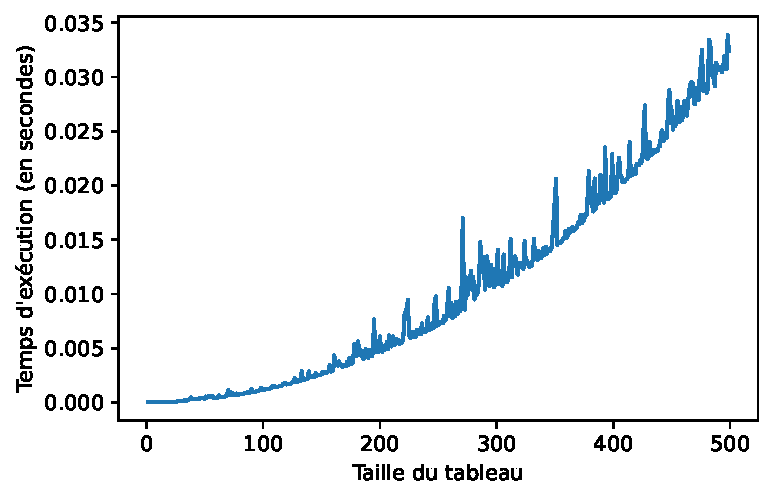
\includegraphics{tris_files/figure-pdf/cell-6-output-1.pdf}

}

\end{figure}

\hypertarget{tri-par-suxe9lection-1}{%
\subsubsection{Tri par sélection}\label{tri-par-suxe9lection-1}}

\begin{Shaded}
\begin{Highlighting}[]
\ImportTok{import}\NormalTok{ timeit}
\ImportTok{import}\NormalTok{ matplotlib.pyplot }\ImportTok{as}\NormalTok{ plt}

\NormalTok{tailles }\OperatorTok{=}\NormalTok{ [i }\ControlFlowTok{for}\NormalTok{ i }\KeywordTok{in} \BuiltInTok{range}\NormalTok{(}\DecValTok{1}\NormalTok{, }\DecValTok{500}\NormalTok{)]}
\NormalTok{temps }\OperatorTok{=}\NormalTok{ []}
\CommentTok{\# on applique le tri dans le pire des cas : tableau trié dans l\textquotesingle{}ordre décroissant}
\ControlFlowTok{for}\NormalTok{ n }\KeywordTok{in}\NormalTok{ tailles:}
\NormalTok{    temps.append(timeit.timeit(}
        \StringTok{"tri\_selection([n{-}k for k in range(n)])"}\NormalTok{,}
        \BuiltInTok{globals}\OperatorTok{=}\BuiltInTok{globals}\NormalTok{(),}
\NormalTok{        number}\OperatorTok{=}\DecValTok{1}
\NormalTok{    ))}
\NormalTok{plt.plot(tailles, temps)}
\NormalTok{plt.xlabel(}\StringTok{"Taille du tableau"}\NormalTok{)}
\NormalTok{plt.ylabel(}\StringTok{"Temps d\textquotesingle{}exécution (en secondes)"}\NormalTok{)}
\NormalTok{plt.show()}
\end{Highlighting}
\end{Shaded}

\begin{figure}[H]

{\centering 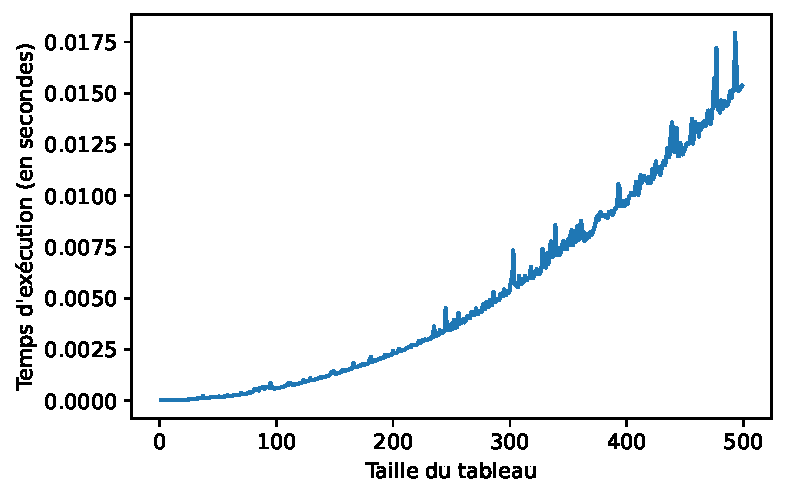
\includegraphics{tris_files/figure-pdf/cell-7-output-1.pdf}

}

\end{figure}

Dans les deux cas, la forme grossièrement parabolique de la courbe est
caractéristique de la complexité quadratique.

\hypertarget{compluxe9ments}{%
\subsection{Compléments}\label{compluxe9ments}}

\href{https://interstices.info/les-algorithmes-de-tri/}{Sur le site
interstices.info} un article très complet sur les algorithmes de tri,
avec des animations pour mieux comprendre.



\end{document}
